\subsection{DPO rewriting with injective rules and matches} 
We focus on DPO rewriting with injective rules and matches. While~\autoref{def:rewriting_inclusion} of injective rewriting rules and rewriting steps may appear more restrictive, they are equivalent to those introduced in \textsection~\ref{sec:dpo}. This equivalence arises because algebraic graph rewriting via double pushouts is defined up to isomorphism. Our preference for these definitions stems from their practical advantage: they provide a clearer view of how the number of monomorphisms from specific graphs changes before and after a rewriting step.
 
\begin{definition}
    \label{def:rewriting_inclusion}
    A rewriting rule $\varphi = (L \overset{l}{\leftarrowtail} K \overset{r}{\rightarrowtail} R)$ consists of two \textbf{inclusions} $l$ and $r$.  
    Two rules $\varphi' = (L' \overset{l'}{\leftarrowtail} K' \overset{r'}{\rightarrowtail} R')$ and $\varphi$ are \textbf{equivalent} if there exist isomorphisms $a,b,c$ such that the commutative diagram illustrated in~\autoref{fig:subgraph_counting:general_rewriting_step_sdfsl_sdfjlsdkjfl} can be constructed:
            \begin{figure}[!ht]
                \centering
                    \resizebox{0.40\textwidth}{!}{
                        \begin{tikzpicture}
                                \node (I) at (0,0) {$K'$};
                                \node (L) at (-2,0) {$L'$};
                                \node (R) at (2,0) {$R'$};
                                \node (G) at (-2,-2) {$L$};
                                \node (C) at (0,-2) {$K$};
                                \node (H) at (2,-2) {$R$};
                                \draw [>->] (I) to  node [midway,below] {$l'$} (L);
                                \draw [>->] (I) to  node [midway,below] {$r'$} (R);
                                \draw [>->] (L) to node [midway,right] {\textbf{a}} (G);
                                \draw [>->] (I) to node [midway,right] {\textbf{b}} (C);
                                \draw [>->] (R) to node [midway,left] {\textbf{c}} (H);
                                \draw [>->] (C) to node [midway,above] {$l$} (G);
                                \draw [>->] (C) to node [midway,above] {$r$} (H);
                                \node [at=($(I)!.5!(G)$)] {$\mathop{=}$};
                                \node [at=($(I)!.5!(H)$)] {$\mathop{=}$};
                            \end{tikzpicture}
                    }
                    \caption{}
                    \label{fig:subgraph_counting:general_rewriting_step_sdfsl_sdfjlsdkjfl}
                \end{figure}
    A rewriting step $G \Rightarrow_\varphi H$ is a double-pushout shown in~\autoref{fig:subgraph_counting:gedfadsdsfdsfds}
%   with injective match $m :L' \rightarrowtail G$:
         \begin{figure}[!ht]
            \centering
          \resizebox{0.40\textwidth}{!}{
              \begin{tikzpicture}
                    \node (I) at (0,0) {$K'$};
                    \node (L) at (-2,0) {$L'$};
                    \node (R) at (2,0) {$R'$};
                    \node (G) at (-2,-2) {$G$};
                    \node (C) at (0,-2) {$C$};
                    \node (H) at (2,-2) {$H$};
                    \draw [>->] (I) to  node [midway,below] {$l'$} (L);
                    \draw [>->] (I) to  node [midway,below] {$r'$} (R);
                    \draw [>->] (L) to node [midway,left] {} (G);
                    \draw [>->] (I) to node [midway,right] { } (C);
                    \draw [>->] (R) to node [midway,left] { } (H);
                    \draw [>->] (C) to node [midway,above] { } (G);
                    \draw [>->] (C) to node [midway,above] { } (H);
                    \node [at=($(I)!.5!(G)$)] {\normalfont PO};
                    \node [at=($(I)!.5!(H)$)] {\normalfont PO};
                  \end{tikzpicture}          }
          \caption{}
          \label{fig:subgraph_counting:gedfadsdsfdsfds}
      \end{figure}
      where all arrows are inclusions and $L' \overset{l'}{\leftarrowtail} K' \overset{r'}{\rightarrowtail} R'$ is equivalent to $\varphi$.
\end{definition}

\subsection{Pre-graphs}
Graphs in double-pushouts that define rewriting steps in \textbf{Graph} can be decomposed into unions of pre-graphs. Pre-graphs model finite directed edge-labeled multigraphs that may contain dangling edges.
\begin{definition}
    \label{def:pre-graph}
    A pre-graph $G$ consists of
    \begin{itemize}
        \item a finite set of nodes, denoted $V(G)$,
        \item a subset $V_{\nexists}(G) \subseteq V(G)$ of missing nodes
        \item a finite set of edges, denoted $E(G)$,
        \item a source function, denoted \( \textbf{src}_G \), (resp. a target function, denoted \( \textbf{dst}_G \)) that assigns to each edge an existing or missing node,
        \item an edge-labeling function, denoted $l_G$, that assigns labels to edges.
    \end{itemize}
\end{definition} 
The set of existing nodes, $V(G) \setminus V_{\nexists}(G)$, is denoted $V_\exists(G)$.

 \begin{example}
    \label{def:pregraph}
     A pre-graph with node-set $\{1,3\}$, a missing node $2$, and 3 dangling edges is illustrated in~\autoref{fig:subgraph_counting:gedfdfssf}.
     \begin{figure}[!ht]
        \centering
        \resizebox{0.5\textwidth}{!}{
        \begin{tikzpicture}
            \graphbox{\(\)}{00mm}{-20mm}{45mm}{20mm}{2mm}{-5mm}{ 
                \coordinate (o) at (-5mm,-8mm); 
                \node[draw,circle] (l1) at ($(o)+(-10mm,0mm)$) {1};
                % \node[draw,circle] (l2) at ($(l1)+(3,0)$) {};
                \node[draw,circle,dashed,red] (l3) at ($(l1)+(1,0)$) {2};
                \node[draw,circle] (l4) at ($(l1)+(2,0)$) {3};
                \draw[->] (l1) edge[bend right]  node[midway,below] {a} (l3);
                \draw[->] (l1) edge[bend left] node[midway,above] {a}  (l3);
                \draw[->] (l3) -- (l4) node[midway,above] {b};
                % \draw[->] (l4) -- (l2) node[midway,above] {a};
            }  
        \end{tikzpicture} 
    }
    \caption{}
    \label{fig:subgraph_counting:gedfdfssf}
    \end{figure}
 \end{example}
 
 A homomorphism of pregraphs is a mapping between two pregraphs that preserves structure and respects missing and existing nodes.
 \begin{definition}[Homomorphism of pre-graphs]
    \label{def:pregraph:homomorphism}
    Let \( G \) and \( H \) be pre-graphs. A \textbf{homomorphism of pre-graphs} $h: G \to H$ consists a pair of functions $h_V: V(G) \to V(H) $ and $h_E: E(G) \to E(H)$ such that
    \begin{itemize}
        \item for every edge \( a \colon s \to t \) in \( G \), the edge \( h_E(a) \) in $H$ has source \( h_V(s) \) and target \( h_V(t) \),
        \item for all $s \in V_{\nexists}(G)$, we have $h_V(s) \in V_{\nexists}(H)$,
        \item for all $t \in V_\exists(G)$, we have $h_V(t) \in V_\exists(H)$.
    \end{itemize} 
\end{definition}

\begin{definition}[Composition]
    \label{def:pregraph:composition}
    Let $f: (G,\lambda) \to (G',\lambda')$ and $g: (G',\lambda') \to (G'',\lambda'')$ be homomorphisms of pre-graphs. Their composition, denoted $g \circ f$, is the homomorphism defined by the component-wise composition of functions $g_V \circ f_V$ and $g_E \circ f_E$.
\end{definition}

We define two operations on pre-graphs that will be used in the following discussion.
The \textbf{union} $C \cup R$ of two sub pre-graphs $C \subseteq G$ and $R \subseteq G$ is a pre-graph with 
\begin{itemize}
    \item Node set: $ V(C) \cup V(R) $,
    \item Missing nodes:
        $(
            V_{\nexists}(C) \cup V_{\nexists}(R)) \setminus 
            (   V_\exists(C) \cup 
             V_\exists(R)  
                   )$
    \item Edge set: $ E(C) \cup E(R) $, 
    \item Source function: $ \opn{src}_C \cup \opn{src}_R $,  
    \item Target function: $ \opn{dst}_C \cup \opn{dst}_R $,  
    \item Edge-labeling function: $ l_C \cup l_R $.   
\end{itemize} 
An example is illustrated in~\autoref{fig:subgraph_counting:union_of_pregraphs}.
\begin{figure}[!ht]
    \centering
    \resizebox{\textwidth}{!}{
        \begin{tikzpicture}  
            \graphbox{\( R \)}{91mm}{-22mm}{45mm}{25mm}{2mm}{2mm}{
                \coordinate (o) at (-5mm,-8mm); 
                \node[draw,circle] (l1) at ($(o)+(-10mm,0mm)$) {1};
                \node[draw,circle] (l2) at ($(l1)+(3,0)$) {2};
                \node[draw,circle] (l3) at ($(l1) + (1,0)$) {4};
                \node[draw,circle] (l4) at ($(l1) + (2,0)$) {5};
                \draw[->] (l1) -- (l3) node[midway,above] {a};
                \draw[->] (l3) -- (l4) node[midway,above] {b};
                \draw[->] (l4) -- (l2) node[midway,above] {a};
            }    
        
            \graphbox{\( C  \)}{0mm}{-22mm}{34mm}{25mm}{2mm}{-3mm}{
                \coordinate (o) at (0mm,-6mm); 
                \node[draw,circle,dashed] (l1) at ($(o)+(-10mm,0mm)$) {1};
                \node[draw,circle,dashed] (l2) at ($(l1)+(2,0)$) {2};
                \node[draw,circle] (l4) at ($(l2) + (0,-1)$) {6};
                \draw[->] (l2) -- (l4) node[midway,right] {a};
                \draw[->] (l2) edge[out=-135,in=-45]node[midway,below] {a} (l1) ;
                % \node[ draw,circle] (l6) at ($(l1) + (0,-1)$) {7};
                % \draw[<-] (l1) -- (l6) node[midway,left] {a};
            }    

            \graphbox{\(C \cup R \)}{40mm}{-22mm}{45mm}{25mm}{2mm}{-3mm}{
                \coordinate (o) at (-5mm,-6mm); 
                \node[draw,circle] (l1) at ($(o)+(-10mm,0mm)$) {1};
                \node[draw,circle] (l2) at ($(l1)+(3,0)$) {2};
                \node[draw,circle] (l3) at ($(l1) + (1,0)$) {4};
                \node[draw,circle] (l4) at ($(l1) + (2,0)$) {5};
                \node[ draw,circle] (l5) at ($(l2) + (0,-1)$) {6};
                % \node[ draw,circle] (l6) at ($(l1) + (0,-1)$) {7};
                % \draw[<-] (l1) -- (l6) node[midway,left] {a};
                \draw[->] (l1) -- (l3) node[midway,above] {a};
                \draw[->] (l3) -- (l4) node[midway,above] {b};
                \draw[->] (l4) -- (l2) node[midway,above] {a};
                \draw[->] (l2) -- (l5) node[midway,right] {a};
                \draw[->] (l2) edge[out=-135,in=-45]node[midway,below] {a} (l1) ;
            }    
             
        \end{tikzpicture}
    }
    \caption{Union of pre-graphs}
    \label{fig:subgraph_counting:union_of_pregraphs}
    \end{figure}


    % \textcolor{red}{Intersection} $G \cap H$: 
    % \vspace{1mm}

    % % \begin{center}
    %     \resizebox{0.95\textwidth}{!}{
    %     \begin{tikzpicture}
    %         \graphbox{\( G \)}{0mm}{-22mm}{34mm}{26mm}{2mm}{-3mm}{
    %             \coordinate (o) at (0mm,-6mm); 
    %             \node[draw,circle] (l1) at ($(o)+(-10mm,0mm)$) {1};
    %             \node[draw,circle] (l2) at ($(l1)+(2,0)$) {2};
    %             \node[draw,circle] (l3) at ($(l1) + (1,0)$) {3};
    %             \node[draw,circle] (l4) at ($(l2) + (0,-1)$) {6};
    %             \draw[->] (l1) -- (l3) node[midway,above] {a};
    %             \draw[->] (l3) -- (l2) node[midway,above] {a};
    %             \draw[->] (l2) -- (l4) node[midway,right] {a};
    %             \node[draw,circle] (l6) at ($(l1) + (0,-1)$) {7};
    %             \draw[<-] (l1) -- (l6) node[midway,left] {a};
    %             \draw[->] (l2) edge[out=-135,in=-45]node[midway,below] {a} (l1) ;
    %         }    
    
    %         \graphbox{ \textcolor{red}{\(G \cap H\)}  }{40mm}{-22mm}{34mm}{25mm}{2mm}{-3mm}{
    %             \coordinate (o) at (0mm,-6mm); 
    %             \node[draw,circle] (l1) at ($(o)+(-10mm,0mm)$) {1};
    %             \node[draw,circle] (l2) at ($(l1)+(2,0)$) {2};
    %             \node[draw,circle] (l4) at ($(l2) + (0,-1)$) {6};
    %             \draw[->] (l2) -- (l4) node[midway,right] {a};
    %             \draw[->] (l2) edge[out=-135,in=-45]node[midway,below] {a} (l1) ;
    %             \node[ draw,circle] (l6) at ($(l1) + (0,-1)$) {7};
    %             \draw[<-] (l1) -- (l6) node[midway,left] {a};
    %         }    
    
    %         \graphbox{\( H \)}{80mm}{-22mm}{45mm}{25mm}{2mm}{-6mm}{
    %             \coordinate (o) at (-5mm,-3mm); 
    %             \node[draw,circle] (l1) at ($(o)+(-10mm,0mm)$) {1};
    %             \node[draw,circle] (l2) at ($(l1)+(3,0)$) {2};
    %             \node[draw,circle] (l3) at ($(l1) + (1,0)$) {4};
    %             \node[draw,circle] (l4) at ($(l1) + (2,0)$) {5};
    %             \node[ draw,circle] (l5) at ($(l2) + (0,-1)$) {6};
    %             \node[ draw,circle] (l6) at ($(l1) + (0,-1)$) {7};
    %             \draw[<-] (l1) -- (l6) node[midway,left] {a};
    %             \draw[->] (l1) -- (l3) node[midway,above] {a};
    %             \draw[->] (l3) -- (l4) node[midway,above] {b};
    %             \draw[->] (l4) -- (l2) node[midway,above] {a};
    %             \draw[->] (l2) -- (l5) node[midway,right] {a};
    %             \draw[->] (l2) edge[out=-135,in=-45]node[midway,below] {a} (l1) ;
    %         }    
           
    %         % \node () at (37mm,-33mm) {\( \leftarrowtail \)};
    %         % \node () at (77mm,-33mm) {\( \rightarrowtail \)}; % C -> H
    %     \end{tikzpicture}
    %     }         
    % \end{center}
The \textbf{relative complement} of $R$ in $H$ where $R \subseteq H$, denoted $H \setminus R$, is the pre-graph with
\begin{itemize}
    \item Edges $X = E(H) \setminus E(R)$,
    \item Nodes $Y =  \bigcup \{\{\opn{src}(e), \opn{dst}(e)\} \mid e \in X \}$ where $\bigcup$ returns the union of all sets in the set,  
    \item Missing nodes $
   ( V_{\nexists}(H)  \cup
        (
                  V_\exists(H) 
                  \cap 
                  V_\exists(R)
                  )
   )
        \cap  
        Y
                  $,
    \item Source function: ${\opn{src}_H}$ restricted to $X$,
    \item Target function: ${\opn{dst}_H}$ restricted to $X$,
    \item Edge-labeling function : $l_H$ restricted to $X$.
\end{itemize}
An example is shown in~\autoref{fig:subgraph_counting:relative_complement_of_pregraphs}.
    \begin{figure}[!ht]
        \centering
  \resizebox{\textwidth}{!}{
        \begin{tikzpicture}  
            \phantom{
                \graphbox{\( G \)}{0mm}{-22mm}{34mm}{22mm}{2mm}{-3mm}{
                }  
            }
            \graphbox{\( R \)}{80mm}{-22mm}{45mm}{25mm}{2mm}{2mm}{
                \coordinate (o) at (-5mm,-8mm); 
                \node[draw,circle] (l1) at ($(o)+(-10mm,0mm)$) {1};
                \node[draw,circle] (l2) at ($(l1)+(3,0)$) {2};
                \node[draw,circle] (l3) at ($(l1) + (1,0)$) {4};
                \node[draw,circle] (l4) at ($(l1) + (2,0)$) {5};
                \draw[->] (l1) -- (l3) node[midway,above] {a};
                \draw[->] (l3) -- (l4) node[midway,above] {b};
                \draw[->] (l4) -- (l2) node[midway,above] {a};
            }    
        
            \graphbox{\( H \setminus R  \)}{40mm}{-22mm}{34mm}{25mm}{2mm}{-3mm}{
                \coordinate (o) at (0mm,-6mm); 
                \node[draw,dashed,circle] (l1) at ($(o)+(-10mm,0mm)$) {1};
                \node[draw,dashed,circle] (l2) at ($(l1)+(2,0)$) {2};
                \node[draw,circle] (l4) at ($(l2) + (0,-1)$) {6};
                \draw[->] (l2) -- (l4) node[midway,right] {a};
                \draw[->] (l2) edge[out=-135,in=-45]node[midway,below] {a} (l1) ;
                % \node[ draw,circle] (l6) at ($(l1) + (0,-1)$) {7};
                % \draw[<-] (l1) -- (l6) node[midway,left] {a};
            }    

            \graphbox{\( H \)}{-11mm}{-22mm}{45mm}{25mm}{2mm}{-3mm}{
                \coordinate (o) at (-5mm,-6mm); 
                \node[draw,circle] (l1) at ($(o)+(-10mm,0mm)$) {1};
                \node[draw,circle] (l2) at ($(l1)+(3,0)$) {2};
                \node[draw,circle] (l3) at ($(l1) + (1,0)$) {4};
                \node[draw,circle] (l4) at ($(l1) + (2,0)$) {5};
                \node[ draw,circle] (l5) at ($(l2) + (0,-1)$) {6};
                % \node[ draw,circle] (l6) at ($(l1) + (0,-1)$) {7};
                % \draw[<-] (l1) -- (l6) node[midway,left] {a};
                \draw[->] (l1) -- (l3) node[midway,above] {a};
                \draw[->] (l3) -- (l4) node[midway,above] {b};
                \draw[->] (l4) -- (l2) node[midway,above] {a};
                \draw[->] (l2) -- (l5) node[midway,right] {a};
                \draw[->] (l2) edge[out=-135,in=-45]node[midway,below] {a} (l1) ;
            }    
            % \node () at (102mm,-18mm) {\( \downarrowtail \)};
            % \node () at (77mm,-33mm) {\( \rightarrowtail \)}; % C -> H
        \end{tikzpicture}
    }
    \caption{Relative complement of pre-graphs}
    \label{fig:subgraph_counting:relative_complement_of_pregraphs}
    \end{figure}

 
\subsection{$X$-occurrences}
Consider a rewriting step illustrated by the left diagram in~\autoref{def:x_occurrence}.
Since all arrows are inclusions, by~\autoref{def:rewriting_inclusion}, graphs can be decomposed as unions of pre-graphs. This decomposition yields the the right diagram of~\autoref{def:x_occurrence}, where $K, L', R',C'$ are pre-graphs and $L = L' \cup K$, $R = R' \cup K$, $C = C' \cup K$, $G = L' \cup K \cup C'$, $H = R' \cup K \cup C'$.
   \begin{definition}
    \label{def:x_occurrence}
    A double pushout diagram illlustrated in~\autoref{fig:subgraph_counting:pushoutsquare} can be decomposed into the diagram illustrated in~\autoref{fig:subgraph_counting:decomposition_of_rewriting_step}.
    \begin{figure}[!ht]
        \centering
       \resizebox{0.49\textwidth}{!}{
        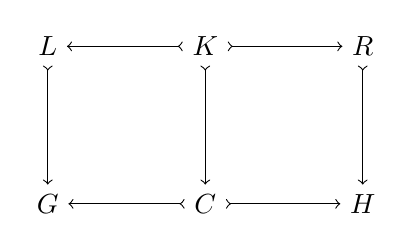
\begin{tikzpicture}
            % [node distance=15mm]
            \node (I) at (0,0) {$K$};
            \node (L)  at (-2,0) {$L$};
            \node (R)  at (2,0) {$R$};
            \node (G)  at (-2,-2) {$G$};
            \node (C)  at (0,-2) {$C$};
            \node (H)  at (2,-2) {$H$};
            \draw [>->] (I) to  node [midway,below] { } (L);
            \draw [>->] (I) to  node [midway,below] { } (R);
            \draw [>->] (L) to node [midway,right] { } (G);
            \draw [>->] (I) to  node [midway,right] 
            % {$u$}
            {} (C);
            \draw [>->] (R) to  node [midway,right] 
            {}
            (H);
            \draw [>->] (C) to node [midway,above] {} (G);
            \draw [>->] (C) to node [midway,above] 
            {}
            (H);
            % \node [at=($(I)!.5!(G)$)] {\normalfont PO};
            % \node [at=($(I)!.5!(H)$)] {\normalfont PO};
        \end{tikzpicture}
    }
    \caption{}
    \label{fig:subgraph_counting:pushoutsquare}
    \end{figure}
    \begin{figure}[!ht]
        \centering
    \resizebox{0.49\textwidth}{!}{
            \begin{tikzpicture} 
                \coordinate (k) at (0, 0);
                \draw[fill=white] ($(k)+(0,0)$) rectangle ($(k)+(0.5,0.5)$);
                \node () at ($(k)+(0.25,0.25)$) {\( \mathrm{K} \)};
            
                \coordinate (c) at (0, -2.2);
                \draw[fill=blue!20]
                ($(c)+(0,-0.5)$)
                -- ($(c)+(0,0.5)$) 
                -- ($(c)+(1,0.5)$) 
                arc[start angle=0, end angle=-90, radius=1]
                -- cycle;
                \node () at ($(c)+(0.75,0.25)$) {\( \mathrm{C'} \)};
                \draw[fill=white] ($(c)+(0,0)$) rectangle ($(c)+(0.5,0.5)$);
                \node () at ($(c)+(0.25,0.25)$) {\( \mathrm{K} \)};
            
                \coordinate (l) at (-3, 0);
                \draw[fill=orange!20] ($(l)+(-0.5,0)$) rectangle ($(l)+(0.5,1)$);
                \node () at ($(l)+(-0.23,0.25)$) {\( \mathrm{L'} \)};
                \draw[fill=white] ($(l)+(0,0)$) rectangle ($(l)+(0.5,0.5)$);
                \node () at ($(l)+(0.25,0.25)$) {\( \mathrm{K} \)};
            
                \coordinate (g) at (-3, -2.2);
                \draw[fill=blue!20]
                ($(g)+(0,-0.5)$)
                -- ($(g)+(0,0.5)$)
                -- ($(g)+(1,0.5)$) 
                arc[start angle=0, end angle=-90, radius=1]
                -- cycle;
                \draw[fill=orange!20] ($(g)+(-0.5,0)$) rectangle ($(g)+(0.5,1)$);
                \node () at ($(g)+(0.75,0.25)$) {\( \mathrm{C'} \)};
                \node () at ($(g)+(-0.23,0.25)$) {\( \mathrm{L'} \)};
                \draw[fill=white] ($(g)+(0,0)$) rectangle ($(g)+(0.5,0.5)$);
                \node () at ($(g)+(0.25,0.25)$) {\( \mathrm{K} \)};
            
                \coordinate (r) at (3,0);
                \draw[fill=red!20] ($(r)+(-0.5,0)$)
                -- ($(r)+(-0.5,0.5)$)
                -- ($(r)+(0,1)$)
                --  ($(r)+(0.5,1)$)
                -- ($(r)+(0.5,0)$)
                -- cycle;
                \node () at ($(r)+(-0.23,0.25)$) {\( \mathrm{R'} \)};
                \draw[fill=white] ($(r)+(0,0)$) rectangle ($(r)+(0.5,0.5)$);
                \node () at ($(r)+(0.25,0.25)$) {\( \mathrm{K} \)};
            
                \coordinate (h) at (3, -2.2);
                \draw[fill=blue!20]
                ($(h)+(0,-0.5)$)
                -- ($(h)+(0,0.5)$)
                -- ($(h)+(1,0.5)$) 
                arc[start angle=0, end angle=-90, radius=1]
                -- cycle;
                \draw[fill=red!20] ($(h)+(-0.5,0)$)
                -- ($(h)+(-0.5,0.5)$)
                -- ($(h)+(0,1)$)
                --  ($(h)+(0.5,1)$)
                -- ($(h)+(0.5,0)$)
                -- cycle;
            \node () at ($(h)+(0.75,0.25)$) {\( \mathrm{C'} \)};
            \draw[fill=white] ($(h)+(0,0)$) rectangle ($(h)+(0.5,0.5)$);
            \node () at ($(h)+(0.25,0.25)$) {\( \mathrm{K} \)};
            \node () at ($(h)+(-0.23,0.25)$) {\( \mathrm{R'} \)};
            
                \node[ font=\huge] (kl) at ($(k)!0.5!(l)+(0.25,0.25)$)
            %    {\( \overset{l}{\leftarrowtail} \)}
                {\( \leftarrowtail \)}
                ; 
                \node[ font=\huge] (kr) at ($(k)!0.5!(r)+(0.25,0.25)$)
                {\( \rightarrowtail \)}
                ;  
                \node[ font=\huge] (cg) at ($(c)!0.5!(g)+(0.25,0.25)$) 
                {\( \leftarrowtail \)}
            ;  
                \node[ font=\huge] (ch) at ($(c)!0.5!(h)+(0.25,0.25)$)
                {\( \rightarrowtail \)}
            ; 
                \node[ font=\huge] (kc) at ($(k)!0.5!(c)+(0.2,0.4)$) {\( \downarrowtail \)}; 
            %   \node[ font=\LARGE] () at ($(l)!0.5!(g)+(0.5,0.4)$) {$m$}; 
                \node[ font=\huge] (lg) at ($(l)!0.5!(g)+(0.1,0.4)$) {\( \downarrowtail \)}; 
                \node[ font=\huge] (rh) at ($(r)!0.5!(h)+(0.1,0.4)$) {\( \downarrowtail \)}; 
            %   \node[ font=\LARGE] () at ($(r)!0.5!(h)+(0.55,0.4)$) {$m'$}; 
            %   \node[ font=\LARGE] () at ($(k)!0.5!(c)+(0.5,0.4)$) {$u$}; 
            \end{tikzpicture}
          }
        \caption{}
        \label{fig:subgraph_counting:decomposition_of_rewriting_step}
   \end{figure}
     Let $X$ be a subgraph of $L$.  An \textbf{$X$-occurrence} in a graph $G$ is an \textbf{monomorphism} from $X$ to $G$. An $X$-occurrence in $G$ is 
    \begin{itemize}
        \item \textbf{shared} if its image is included in $C$,
        \item \textbf{explicit} if its image is  included in $L$,
        \item \textbf{implicit} if its image has elements in both $C'$ and $L'$.
    \end{itemize}  
    An $X$-occurrence in $H$ is 
    \begin{itemize}
        \item \textbf{shared} if its image is included in $C$,
        \item \textbf{explicit} if its image is included in $R$,
        \item \textbf{implicit} if its image has elements in both $C'$ and $R'$.
    \end{itemize} 

    Intuitively, the rewriting step implicitly creates the implicit $X$-occurrences in $H$ and implicitly destroys implicit $X$-occurrences in $G$. Given an implicit $X$-occurrence $x$ in $H$, its image can be decomposed as the union $R_x \cup C_x$, where $R_x = \opn{Im}(x) \cap R$ (the part of the image overlapping the right-hand side R ), and $C_x = \opn{Im}(x) \cap C$ (the part overlapping the context C ). For every graph monomorphism $h : R_x \rightarrowtail L$ that preserves interface elements (i.e., \( h(k) = k \) for all \( k \in K \)), we define the \textbf{corresponding $X$-occurrence of $x$ relative to $h$} as the $X$-occurrence $y$ in $G$ given by:
        $$
        y(z) = 
        \begin{cases}
        z & \text{if } z \in x^{-1}(C_x), \\
        h(x(z)) & \text{if } z \in x^{-1}(R_x \setminus C_x).
        \end{cases}
        $$
   \end{definition} 



% \begin{definition}
%     \label{def:corresponding_occurrence}
%      An \textbf{$X$-occurrence} in $G$ is a subgraph of $G$ isomorphic to $X$. An \textbf{$X$-occurrence $x$ implicitly created by the rewriting step} is an \( X \)-occurrence in $H$ which is included neither in \( R \) nor in $C$. 
%       The occurrence $x$ can be decomposed as the union of graphs $x = R_x \cup C_x$ where $R_x = x \cap R$ and $C_x = x \cap C$. For every graph monomorphism $h : R_x \rightarrowtail L$ that preserves interface elements (i.e., \( h(k) = k \) for all \( k \in K \)), we define the \textbf{corresponding $X$-occurrence of $x$ relative to $h$} as the $X$-occurrence in $G$ given by $h(R_x) \cup C_x$.
%     An \textbf{$X$-occurrence implicitly destroyed by the rewriting step} is an \( X \)-occurrence in $G$ which is included neither in \( L \) nor in $C$.
% \end{definition}


\begin{example}
    Let $X$ be the graph
\tikz[baseline=-0.5ex]{ 
        \node[draw,circle] (x) at (0,0) {};  
        \node[draw,circle] (y) at (1,0) {};
        \node[draw,circle] (z) at (2,0) {};
        \draw[->] (x) -- node[midway,above] {a} (y) ;
        \draw[->] (y) -- node[midway,above] {a} (z) ;
}.
Consider the $X$-occurrences in the decomposition of a rewriting step using the rule in~\autoref{ex:grsaa} shown in~\autoref{fig:subgraph_counting:occurrdlfdjslfkjsa}.
    \begin{figure} 
      \centering
      \resizebox{0.7\textwidth}{!}{
      \begin{tikzpicture}
          \graphbox{$L$}{0mm}{0mm}{34mm}{15mm}{2mm}{-5mm}{
              \coordinate (o) at (0mm,-3mm); 
              \node[draw,circle] (l1) at ($(o)+(-10mm,0mm)$) {1};
              \node[draw,circle] (l2) at ($(l1)+(2,0)$) {2};
              \node[draw,circle] (l3) at ($(l1) + (1,0)$) {3};
              \draw[->] (l1) -- (l3) node[midway,above] {a};
              \draw[->] (l3) -- (l2) node[midway,above] {a};
          }     
          \graphbox{$K$}{40mm}{0mm}{24mm}{15mm}{2mm}{-5mm}{
              \coordinate (o) at (5mm,-3mm); 
              \node[draw,circle] (l1) at ($(o)+(-10mm,0mm)$) {1};
              \node[draw,circle] (l2) at ($(l1)+(1,0)$) {2};
              % \node[draw,circle] (l3) at ($(l1) + (1,0)$) {$\ $};
              % \draw[->] (l1) -- (l3) node[midway,above] {a};
              % \draw[->] (l3) -- (l2) node[midway,above] {a};
          }    
          \graphbox{$R$}{70mm}{0mm}{45mm}{15mm}{2mm}{-5mm}{
              \coordinate (o) at (-5mm,-3mm); 
              \node[draw,circle] (l1) at ($(o)+(-10mm,0mm)$) {1};
              \node[draw,circle] (l2) at ($(l1)+(3,0)$) {2};
              \node[draw,circle] (l3) at ($(l1) + (1,0)$) {4};
              \node[draw,circle] (l4) at ($(l1) + (2,0)$) {5};
              \draw[->] (l1) -- (l3) node[midway,above] {a};
              \draw[->] (l3) -- (l4) node[midway,above] {b};
              \draw[->] (l4) -- (l2) node[midway,above] {a};
          }    
          \node () at (37mm,-8mm) {$\overset{l}{\leftarrowtail}$};
          \node () at (67mm,-8mm) {$\overset{r}{\rightarrowtail}$};
          % \draw[>->] (51mm,2mm) -- (52mm,3mm);
      \end{tikzpicture}
      }
      \caption{}
      \label{fig:subgraph_counting:occurrdlfdjslfkjsa}
  \end{figure}
    This decomposition is illustrated in~\autoref{fig:subgraph_counting:occurrendfsdadsgces_of_x} using the visual notation for graph homomorphisms introduced in~\autoref{notation:graph_homomorphism}, with distinct pre-graphs highlighted in different colors.
\begin{figure}[!ht]
    \centering
    \resizebox{0.8\textwidth}{!}{
      \begin{tikzpicture}
              \graphbox{\( L = L' \cup K \)}{0mm}{5mm}{34mm}{20mm}{2mm}{-5mm}{
                  \coordinate (o) at (0mm,-8mm); 
                  \node[draw,circle] (l1) at ($(o)+(-10mm,0mm)$) {1};
                  \node[draw,circle] (l2) at ($(l1)+(2,0)$) {2};
                  \node[orange,draw,circle] (l3) at ($(l1) + (1,0)$) {3};
                  \draw[orange,->] (l1) -- (l3) node[midway,above] {a};
                  \draw[orange,->] (l3) -- (l2) node[midway,above] {a};
              } 

              \graphbox{\( K \)}{40mm}{5mm}{34mm}{20mm}{2mm}{-5mm}{
                  \coordinate (o) at (0mm,-8mm); 
                  \node[draw,circle] (l1) at ($(o)+(-10mm,0mm)$) {1};
                  \node[draw,circle] (l2) at ($(l1)+(2,0)$) {2};
              }  

              \graphbox{\( R = R' \cup K \)}{80mm}{5mm}{45mm}{20mm}{2mm}{-5mm}{
                  \coordinate (o) at (-5mm,-8mm); 
                  \node[draw,circle] (l1) at ($(o)+(-10mm,0mm)$) {1};
                  \node[draw,circle] (l2) at ($(l1)+(3,0)$) {2};
                  \node[red,draw,circle] (l3) at ($(l1) + (1,0)$) {4};
                  \node[red,draw,circle] (l4) at ($(l1) + (2,0)$) {5};
                  \draw[red,->] (l1) -- (l3) node[midway,above] {a};
                  \draw[red,->] (l3) -- (l4) node[midway,above] {b};
                  \draw[red,->] (l4) -- (l2) node[midway,above] {a};
              }    

              \graphbox{\( G = L' \cup K \cup C' \)}{0mm}{-22mm}{34mm}{30mm}{2mm}{-10mm}{
                  \coordinate (o) at (0mm,-3mm); 
                  \node[draw,circle] (l1) at ($(o)+(-10mm,0mm)$) {1};
                  \node[draw,circle] (l2) at ($(l1)+(2,0)$) {2};
                  \node[draw,circle,orange] (l3) at ($(l1) + (1,0)$) {3};
                  \node[blue, draw,circle] (l4) at ($(l2) + (0,-1)$) {6};
                  \draw[orange,->] (l1) -- (l3) node[midway,above] {a};
                  \draw[orange,->] (l3) -- (l2) node[midway,above] {a};
                  \draw[blue,->] (l2) -- (l4) node[midway,right] {a};
                %   \node[blue,draw,circle] (l6) at ($(l1) + (0,-1)$) {7};
                %   \draw[blue,<-] (l1) -- (l6) node[midway,left] {a};
                \node[blue,draw,circle] (l7) at ($(l4) + (-1,0)$) {7};
                  \draw[blue,->] (l4) -- (l7) node[midway,below] {a};
              }    

              \graphbox{\( C = K \cup C' \)}{40mm}{-22mm}{34mm}{30mm}{2mm}{-10mm}{
                  \coordinate (o) at (0mm,-3mm); 
                  \node[draw,circle] (l1) at ($(o)+(-10mm,0mm)$) {1};
                  \node[draw,circle] (l2) at ($(l1)+(2,0)$) {2};
                  \node[blue,draw,circle] (l4) at ($(l2) + (0,-1)$) {6};
                  \draw[blue,->] (l2) -- (l4) node[midway,right] {a};
                %   \node[blue,draw,circle] (l6) at ($(l1) + (0,-1)$) {7};
                %   \draw[blue,<-] (l1) -- (l6) node[midway,left] {a};
                    \node[blue,draw,circle] (l7) at ($(l4) + (-1,0)$) {7};
                  \draw[blue,->] (l4) -- (l7) node[midway,below] {a};
              }    

              \graphbox{\( H = R' \cup K \cup C' \)}{80mm}{-22mm}{45mm}{30mm}{2mm}{-10mm}{
                  \coordinate (o) at (-5mm,-3mm); 
                  \node[draw,circle] (l1) at ($(o)+(-10mm,0mm)$) {1};
                  \node[draw,circle] (l2) at ($(l1)+(3,0)$) {2};
                  \node[draw,circle,red] (l3) at ($(l1) + (1,0)$) {4};
                  \node[draw,circle,red] (l4) at ($(l1) + (2,0)$) {5};
                  \node[blue,draw,circle] (l5) at ($(l2) + (0,-1)$) {6};
                %   \node[blue,draw,circle] (l6) at ($(l1) + (0,-1)$) {7};
                %   \draw[blue,<-] (l1) -- (l6) node[midway,left] {a};
                  \draw[red,->] (l1) -- (l3) node[midway,above] {a};
                  \draw[red,->] (l3) -- (l4) node[midway,above] {b};
                  \draw[red,->] (l4) -- (l2) node[midway,above] {a};
                  \draw[blue,->] (l2) -- (l5) node[midway,right] {a};
                        \node[blue,draw,circle] (l7) at ($(l5) + (-1,0)$) {7};
                  \draw[blue,->] (l5) -- (l7) node[midway,below] {a};
              }    

              \node () at (37mm,-8mm) {\( \leftarrowtail \)}; % K -> L
              \node () at (77mm,-8mm) {\( \rightarrowtail \)}; % K -> R
              \node () at (17mm,-18mm) {\( m\ \downarrowtail \)};
              \node () at (37mm,-33mm) {\( \leftarrowtail \)};
              \node () at (52mm,-18mm) {\( \downarrowtail \)};
              \node () at (92mm,-18mm) {\( \downarrowtail \)};
              \node () at (77mm,-33mm) {\( \rightarrowtail \)}; % C -> H
      \end{tikzpicture}
      }
      \caption{}
      \label{fig:subgraph_counting:occurrendfsdadsgces_of_x}
   \end{figure}
   There are 
\begin{itemize}
    \item 1 occurrence shared by $G$ and $H$: 
     \tikz[baseline=-0.5ex]{ 
        \node[draw,circle] (x) at (0,0) {2};  
        \node[blue,draw,circle] (y) at (1,0) {6};
        \node[blue,draw,circle] (z) at (2,0) {7};
        \draw[blue,->] (x) -- node[midway,above] {a} (y) ;
        \draw[blue,->] (y) -- node[midway,above] {a} (z) ;
     }
    \item 1 explicit occurrence in $G$:
     \tikz[baseline=-0.5ex]{ 
        \node[draw,circle] (x) at (0,0) {1};  
        \node[orange,draw,circle] (y) at (1,0) {3};
        \node[draw,circle] (z) at (2,0) {2};
        \draw[orange,->] (x) -- node[midway,above] {a} (y) ;
        \draw[orange,->] (y) -- node[midway,above] {a} (z) ;
    }
 
    \item 1 implicit occurrences in $G$:
    \tikz[baseline=-0.5ex]{ 
        \node[orange,draw,circle] (x) at (0,0) {3};  
        \node[draw,circle] (y) at (1,0) {2};
        \node[blue,draw,circle] (z) at (2,0) {6};
        \draw[orange,->] (x) -- node[midway,above] {a} (y) ;
        \draw[blue,->] (y) -- node[midway,above] {a} (z) ;
    } 
 
    \item 0 explicit occurrence in $H$,
    \item 1 implicit occurrences in $H$: 
    \tikz[baseline=-0.5ex]{ 
        \node[red,draw,circle] (x) at (0,0) {5};  
        \node[draw,circle] (y) at (1,0) {2};
        \node[blue,draw,circle] (z) at (2,0) {6};
        \draw[red,->] (x) -- node[midway,above] {a} (y) ;
        \draw[blue,->] (y) -- node[midway,above] {a} (z) ;
}
 
\end{itemize}
    The corresponding X-occurrence of the implicit occurrences \tikz[baseline=-0.5ex]{ 
        \node[red,draw,circle] (x) at (0,0) {5};  
        \node[draw,circle] (y) at (1,0) {2};
        \node[blue,draw,circle] (z) at (2,0) {6};
        \draw[red,->] (x) -- node[midway,above] {a} (y) ;
        \draw[blue,->] (y) -- node[midway,above] {a} (z) ;
} in $H$ relative to the unique monomorphism from 
    \tikz[baseline=-0.5ex]{
      \node[red,draw,circle] (x) at (0,0) {5};
      \node[draw,circle] (y) at (1,0) {2};
      \draw[red,->] (x) -- (y) node[midway, above] {a};
  }
     to 
    \tikz[baseline=-0.5ex]{
      \node[orange,draw,circle] (x) at (0,0) {3};
      \node[draw,circle] (y) at (1,0) {2};
      \draw[orange,->] (x) -- (y) node[midway, above] {a};
  }
    is the implicit occurrences 
       \tikz[baseline=-0.5ex]{ 
        \node[orange,draw,circle] (x) at (0,0) {3};  
        \node[draw,circle] (y) at (1,0) {2};
        \node[blue,draw,circle] (z) at (2,0) {6};
        \draw[orange,->] (x) -- node[midway,above] {a} (y) ;
        \draw[blue,->] (y) -- node[midway,above] {a} (z) ;
    } 
    in $G$.
\end{example}